\documentclass{article}
\usepackage[final]{corl_2024}

\usepackage[T1]{fontenc}
\usepackage[utf8]{inputenc}
\usepackage{lmodern}
\usepackage{microtype}
\usepackage{amsmath}
\usepackage{amssymb}
\usepackage{booktabs}
\usepackage{graphicx}
\usepackage{float}
\usepackage{hyperref}
\usepackage{url}
\usepackage{xcolor}
\usepackage{enumitem}

\title{Final Report: AV Drone Pathing with PPO, SAC, Model-Based RL, and Robustness Modifications}
\author{Leo Shaw \and Siddarth Ashok}
\date{}

\begin{document}
\maketitle

\begin{abstract}
This project studies autonomous quadrotor pathing in a randomized MuJoCo simulation. The task is to navigate from a random initial state to a random 3D goal while avoiding capsule obstacles, respecting a safety envelope, and stabilizing near the target. We evaluate model-free on-policy reinforcement learning with Proximal Policy Optimization (PPO), model-free off-policy reinforcement learning with Soft Actor-Critic (SAC), a preliminary model-based RL result, and two final-project modifications: goal-hover reward shaping and wind-disturbance robustness. Current results show that model-free RL learns meaningful goal-directed and obstacle-aware behavior, but the task remains only partially solved. The best PPO goal-hover policy reaches a mean evaluation return of $366.8$ and a success rate of $45.3\%$, while the wind-trained PPO policy reaches $267.6$ return and $35.9\%$ success under disturbed dynamics.
\end{abstract}

\section{Introduction}
The goal of this project is autonomous drone pathing in a cluttered 3D environment. The environment is a custom MuJoCo quadrotor navigation task implemented in \texttt{jax\_implementation/env.py}. The robot is a simulated Skydio X2-style quadrotor with four thrust actuators. Each episode randomizes the drone's initial state and the target position within a bounded workspace. The environment also randomizes between 1 and 15 capsule obstacles, each roughly 3 meters long. The current workspace bounds are approximately $\pm 6$ m in the horizontal plane and $3.5$ m in altitude. Episodes terminate on success, repeated collision, leaving the safety envelope, excessive speed, numerical failure, or reaching the episode limit.

The policy does not act directly on individual rotor thrusts. Instead, the learned policy outputs a normalized 4D command
\[
a = [v_x, v_y, v_z, \dot{\psi}] \in [-1,1]^4,
\]
where the action specifies desired translational velocity and yaw-rate commands. A low-level proportional controller maps these commands to rotor thrust. This design makes the learned policy responsible for high-level pathing and local motion control, rather than raw attitude stabilization.

Observations are structured as a dictionary containing drone position, velocity, orientation, yaw rate, target position, the relative goal vector, obstacle-relative state, obstacle mask, number of active obstacles, and multiple lidar beam lengths. The lidar beams provide local obstacle detection in several directions; missing lidar hits are clipped to a maximum range. This gives the policy both direct goal geometry and local free-space information.

\paragraph{Reward function.}
The reward is dense and shaped. It includes progress toward the goal, goal-proximity shaping, best-distance improvement, a terminal success bonus, a hover-at-goal reward, lidar/obstacle risk shaping, collision penalties, energy and action-smoothness penalties, speed penalties, and terminal penalties for failure. The final branch also includes a goal-path clearance term from the MBRL branch that penalizes obstacle risk along the straight-line corridor between the drone and the target. Dense shaping was necessary because sparse success-only reward made exploration too difficult under randomized obstacles and continuous quadrotor dynamics.

\section{Methods}
\paragraph{On-policy baseline: PPO.}
The on-policy policy-gradient baseline uses Proximal Policy Optimization (PPO) \cite{schulman2017ppo}. PPO collects fresh rollouts from the current policy and updates the policy using a clipped surrogate objective. PPO was trained in the JAX/Brax pipeline with large-scale parallel simulation, typically using 1024 or 2048 environments on GPU.

\paragraph{Off-policy baseline: SAC.}
The off-policy Q-function baseline uses Soft Actor-Critic (SAC) \cite{haarnoja2018sac}. SAC learns a stochastic actor and soft Q-functions from a replay buffer. This should improve sample efficiency in principle, but in this task SAC was more sensitive to learning rate, replay settings, and late-training policy regression.

\paragraph{Model-based RL: PETS/MPC.}
The merged repository includes a model-based RL implementation under \texttt{jax\_implementation/MBRL/dynamics}. The method is PETS-style ensemble dynamics learning followed by MPC planning with CEM. The dynamics model is pretrained from collected environment data, then updated with online rollouts during MPC evaluation. The current MBRL result available in the repository is an episode cumulative-return curve rather than a full training learning curve, so the main results plot includes it as a provisional estimate scaled to a 2M-step window.

\paragraph{Modification 1: goal-hover reward and termination shaping.}
The first modification targets the main midterm failure case: the drone often moved toward the goal but failed to slow down and remain near it. This modification increases the importance of goal-hover behavior by using a smaller success radius, requiring a short consecutive hover streak for success, increasing the terminal goal reward, strengthening the hover reward, and tuning the landing blend near the target. The goal is to make the learned policy solve the final approach and stabilization phase rather than only learning coarse goal-seeking.

\paragraph{Modification 2: wind-disturbance robustness.}
The second modification introduces wind disturbances during training and evaluation. At reset, each episode samples a wind acceleration vector. During simulation, this wind perturbs the drone's translational velocity at each physics step. The wind is not directly added as an observation, so the policy must learn feedback behavior that corrects drift from state changes. This tests whether the learned pathing policy remains effective under external disturbances rather than only in still-air simulation.

\section{Experimental Results}
Figure~\ref{fig:main-results} shows the current learning curves available in the repository. The figure includes the random-agent baseline, PPO baseline, SAC baseline, Model-based RL, Modification 1, and Modification 2. Each PPO/SAC curve uses only saved evaluation points from its corresponding training run. The model-based RL curve comes from the available cumulative-return data generated by the model-based method.

\begin{figure}[H]
    \centering
    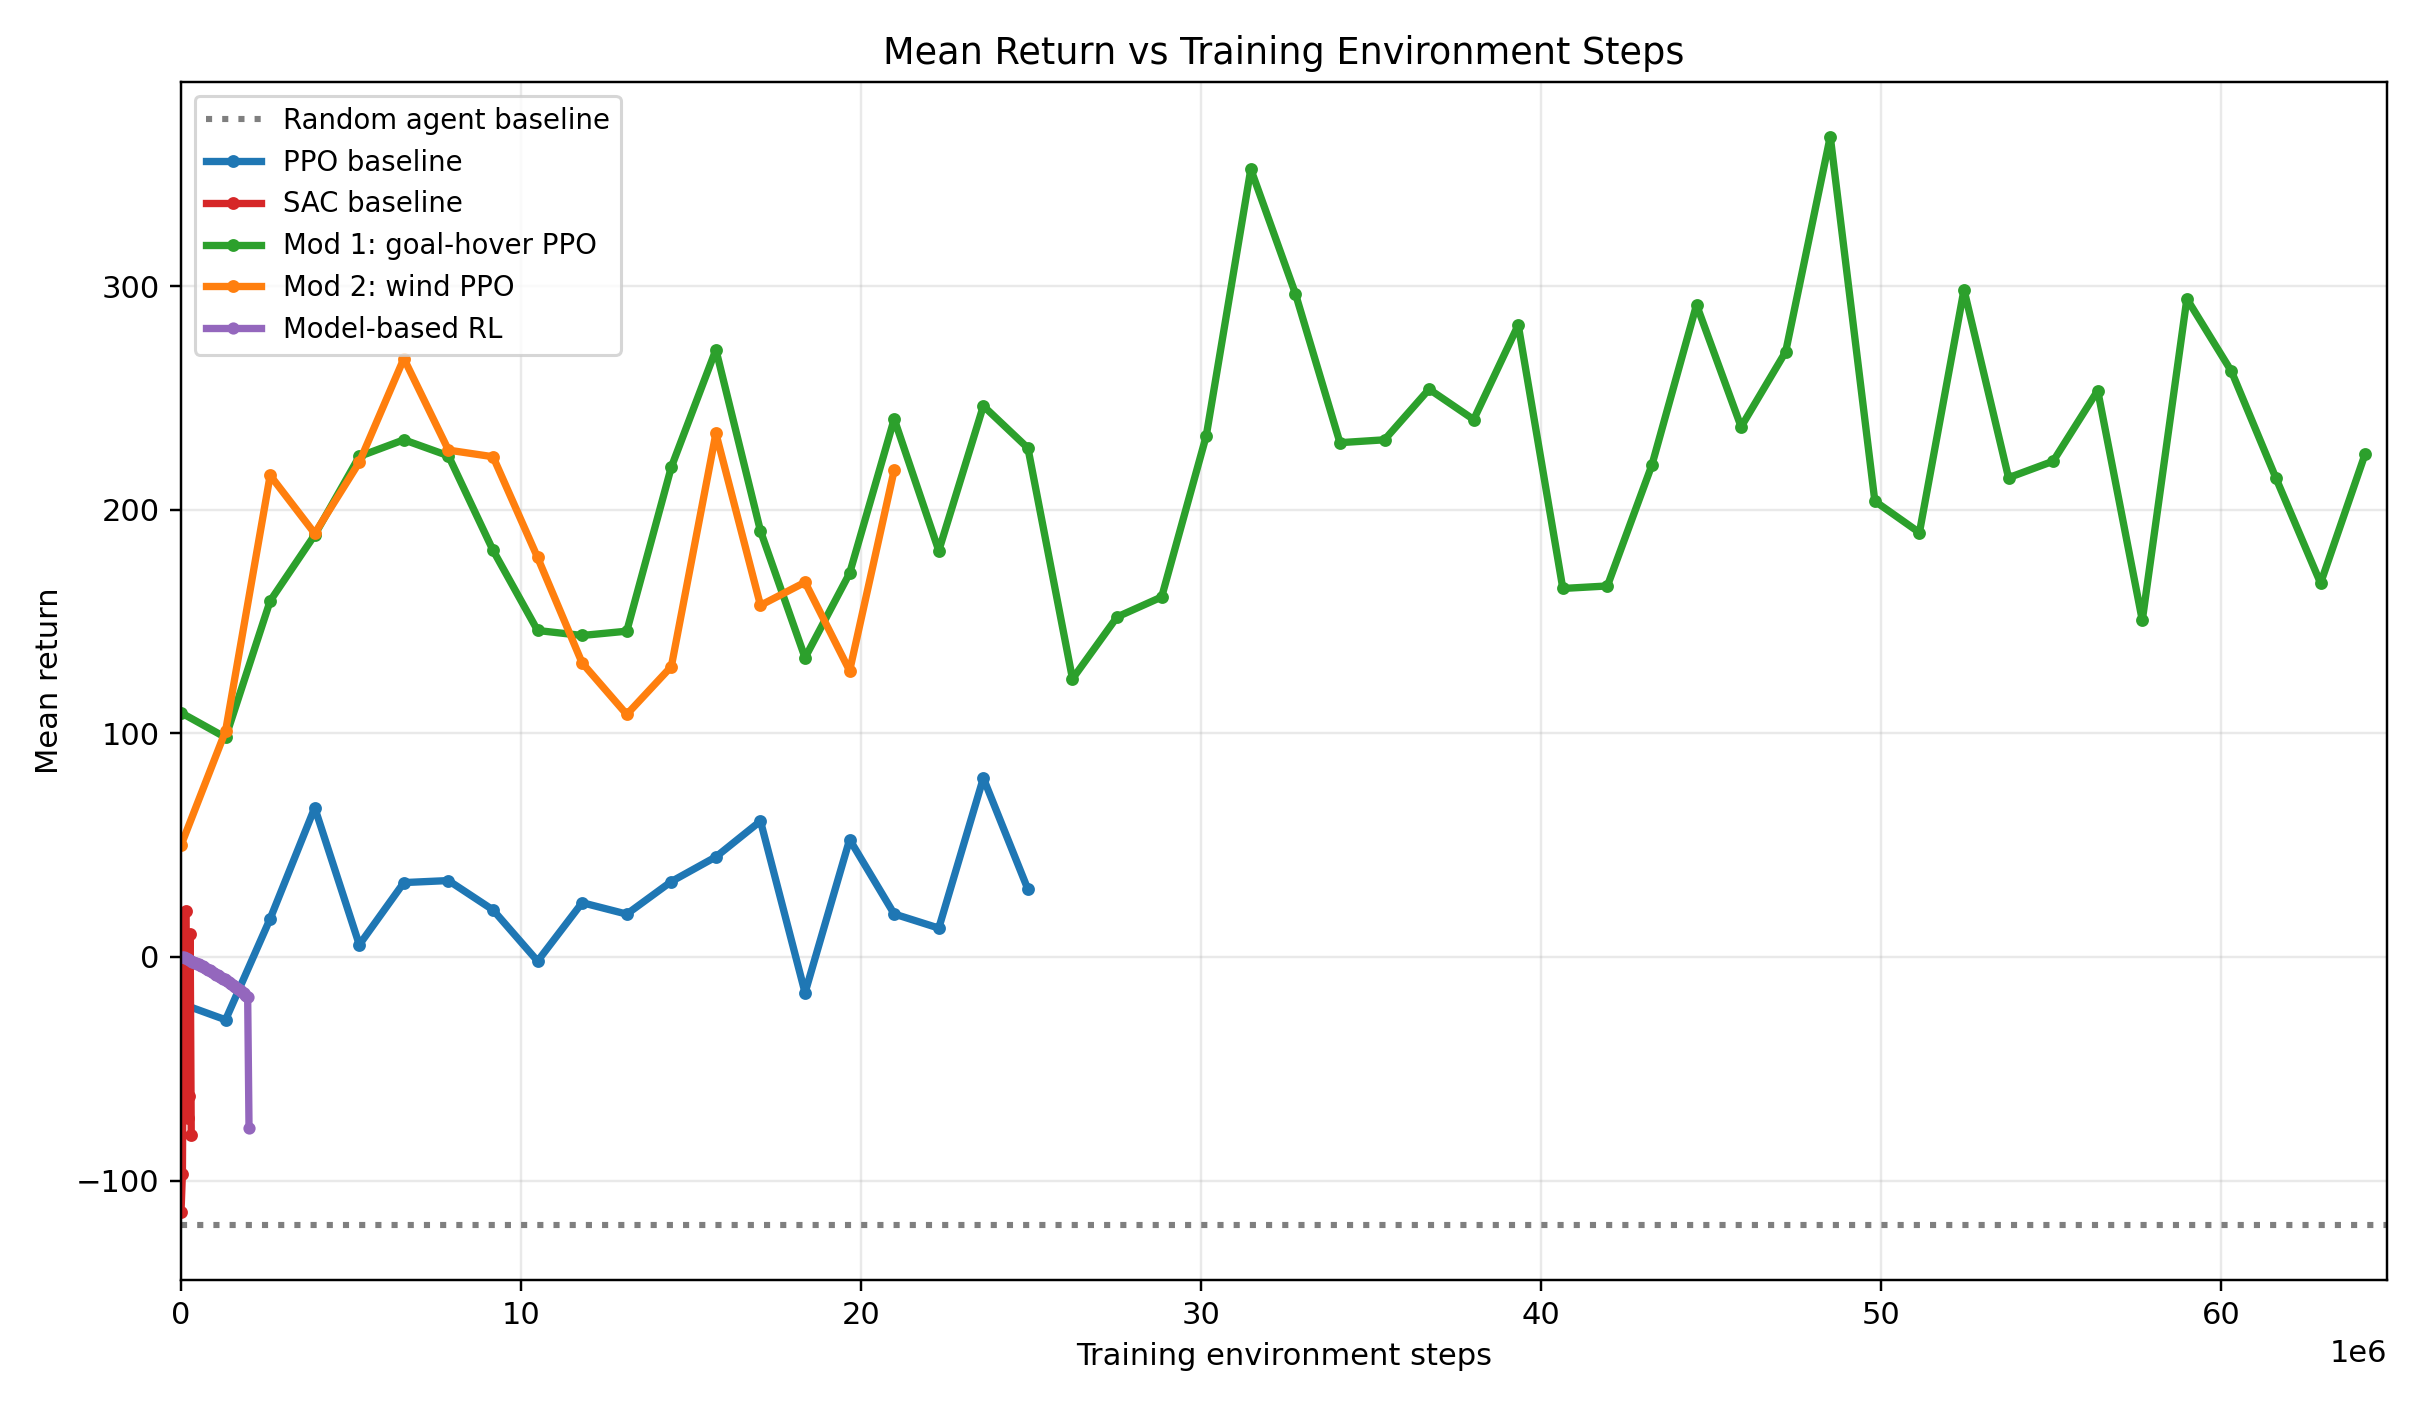
\includegraphics[width=0.97\linewidth]{figs/current_final_results.png}
    \caption{Mean evaluation return versus training environment steps for the random baseline, PPO baseline, SAC baseline, Model-based RL, goal-hover PPO modification, and wind-trained PPO modification.}
    \label{fig:main-results}
\end{figure}

\begin{table}[H]
\centering
\caption{Best checkpoint metrics from current completed runs. Success is the fraction of evaluation episodes satisfying the goal-hover success criterion.}
\label{tab:results}
\begin{tabular}{lrrrr}
\toprule
Method & Best Return & Success & Final Dist. & Collisions \\
\midrule
Random agent & $-120.0$ & $0.0\%$ & -- & -- \\
PPO baseline & $80.0$ & $25.0\%$ & $2.26$ m & $18.23$ \\
SAC baseline & $20.7$ & $18.8\%$ & $2.73$ m & $56.06$ \\
Model-based RL & $-0.1$ & -- & -- & -- \\
Mod 1: goal-hover PPO & $366.8$ & $45.3\%$ & $1.27$ m & $6.05$ \\
Mod 2: wind PPO & $267.6$ & $35.9\%$ & $1.59$ m & $8.28$ \\
\bottomrule
\end{tabular}
\end{table}

\paragraph{Learning curves.}
The baseline PPO curve outperforms the baseline SAC curve, but neither baseline fully solves the task. PPO reaches a best return of about $80.0$, while SAC reaches only about $20.7$ before degrading. Modification 1 produces the strongest completed result, with a best return of $366.8$ and the highest success rate. Modification 2 is lower than the best still-air goal-hover policy, but it remains competitive despite wind disturbances, reaching $267.6$ return and $35.9\%$ success.

\paragraph{Success rates and task metrics.}
The most important task metrics are success rate, final distance to goal, goal-hold streak, and collision count. The baseline PPO succeeds in $25.0\%$ of evaluation episodes, while the baseline SAC succeeds in $18.8\%$. Modification 1 improves success to $45.3\%$ and reduces final distance to $1.27$ m, indicating that goal-hover shaping directly improves the final approach behavior. Modification 2 achieves $35.9\%$ success and $1.59$ m final distance under wind, showing that the policy can compensate for moderate disturbances but loses some performance relative to still-air training.

\paragraph{Failure cases.}
The main failure mode remains final stabilization. Even when the drone makes progress toward the target, it can overshoot, drift through the goal region without maintaining the hover streak, or collide with nearby obstacles during the final approach. A second failure mode is late-training regression: several PPO and SAC runs reached strong intermediate checkpoints and then degraded. This makes best-checkpoint selection important for fair evaluation. For SAC, regression is especially visible: the stable SAC goal-hover run has a final return close to its best checkpoint, but the earlier SAC run degraded substantially after its peak.

\paragraph{Comparison across methods.}
The completed experiments suggest that PPO is the strongest model-free baseline for this environment. SAC can learn useful behavior, but it is more sensitive to hyperparameters and replay dynamics. The goal-hover modification is the clearest improvement over the baseline methods because it attacks the dominant failure mode directly. Wind training produces lower still-air-style reward than the best goal-hover PPO run, but it is solving a harder disturbance-robustness problem and still outperforms the original PPO and SAC baselines.

\paragraph{Comparison across modifications.}
Modification 1 improves nominal task performance more than Modification 2. Goal-hover shaping raises success from $25.0\%$ to $45.3\%$ and reduces final distance from $2.26$ m to $1.27$ m. Modification 2 reaches $35.9\%$ success under wind, which is lower than Modification 1 but still strong given the additional disturbance. The two modifications are complementary: goal-hover shaping improves final stabilization, while wind training improves robustness to external perturbations.

\section{Conclusion and Future Work}
The current experiments show that model-free RL can learn meaningful drone pathing behavior in a randomized MuJoCo quadrotor task, but the task is not fully solved. PPO is the strongest completed baseline, SAC is viable but less stable, and the goal-hover modification produces the best completed policy. The wind modification demonstrates that a policy can remain partially successful under external disturbances. A success rate of roughly $35$--$45\%$ is satisfactory for a course-scale experimental milestone, but it is far below what would be required for deployment-quality autonomous flight.

Before submission, the Model-based RL curve can be replaced with a fuller training-evaluation curve if more evaluation data becomes available. The project website should also be updated with videos for PPO, SAC, MBRL, Modification 1, and Modification 2. Future work should focus on curriculum learning over obstacle count and target distance, stronger final-approach damping, explicit safety constraints, hybrid RL/MPC controllers, and evaluation on held-out obstacle distributions and stronger wind settings.

The project website with videos is available at \url{https://leos-bit.github.io/Intro-to-Robot-Learning-/}. The final version should include videos for all reported agents.

\begin{thebibliography}{9}
\bibitem{schulman2017ppo}
John Schulman, Filip Wolski, Prafulla Dhariwal, Alec Radford, and Oleg Klimov.
Proximal Policy Optimization Algorithms.
\emph{arXiv:1707.06347}, 2017.

\bibitem{haarnoja2018sac}
Tuomas Haarnoja, Aurick Zhou, Pieter Abbeel, and Sergey Levine.
Soft Actor-Critic: Off-Policy Maximum Entropy Deep Reinforcement Learning with a Stochastic Actor.
\emph{International Conference on Machine Learning}, 2018.
\end{thebibliography}

\appendix
\section{Open Final-Report Checklist}
\begin{itemize}[leftmargin=1.2em]
    \item Replace the current Model-based RL curve with a fuller training-evaluation curve if one becomes available.
    \item Add MBRL success rate, final distance, and failure analysis if those evaluation metrics become available.
    \item Update the website with videos for PPO, SAC, MBRL, Modification 1, and Modification 2.
    \item Replace the provisional random-agent constant line if a larger measured random baseline is generated.
\end{itemize}

\end{document}
